\documentclass[11pt,a4paper, twocolumn,
swedish, english %% Make sure to put the main language last!
]{article}
\pdfoutput=1

%% Andréas's custom package 
%% (Will work for most purposes, but is mainly focused on physics.)
\usepackage{custom_as}

%% Figures can now be put in a folder: 
\graphicspath{ {figures/} {figures/water/}%{some_folder_name/}
}

%% If you want to change the margins for just the captions
\usepackage[size=small]{caption}

%% To add todo-notes in the pdf
\usepackage[%disable  %%this will hide all notes
]{todonotes} 

%% Change the margin in the documents
\usepackage[
             top    = 3.5cm,              %% top margin
             bottom = 3.5cm,              %% bottom margin
             left   = 2.2cm, right  = 2.2cm %% left and right margins
]{geometry}


%% If you want to change the formatting of the section headers
%\renewcommand{\thesection}{...}



%%%%%%%%%%%%%%%%%%%%%%%%%%%%%%%%%%%%%%%%%%%%%%%%%%%%%%%%%%%%%%%%%%%%%%
\begin{document}%% v v v v v v v v v v v v v v v v v v v v v v v v v v
%%%%%%%%%%%%%%%%%%%%%%%%%%%%%%%%%%%%%%%%%%%%%%%%%%%%%%%%%%%%%%%%%%%%%%

%%%%%%%%%%%%%%%%%%%% vvv Internal title page vvv %%%%%%%%%%%%%%%%%%%%%

\title{A qualitative investigation of self-diffusion in wet
  paper using the NMR pulse echo method} 
\author{Andréas Sundström \and Tan Qin Yuan}
\date{\today}

\twocolumn[
\begin{@twocolumnfalse}
\maketitle
\begin{abstract}

\end{abstract}
%\tableofcontents
\end{@twocolumnfalse}
]
%\clearpage
%%%%%%%%%%%%%%%%%%%% ^^^ Internal title page ^^^ %%%%%%%%%%%%%%%%%%%%%
%% If you want a list of all todos
%\todolist



\section{Introduction}

As demands for increased rate of recycling and decreased use of fossil
products paper is a good alternative material for e.g. packaging
products, where the recycling rate of paper based packaging is as high
as 82\,\% in Sweden~\cite{Adolfson_NVV2016}. An increase in e-commerce
in the EU~\cite{eurostat_e-commerce2017} and other developed countries
also raises the demand for light-weight and durable cardboard
packaging~\cite{Nordstrand2003}. One major weakness of paper based 
packaging is however susceptibility to water damage which
significantly weakens the strength of the container; studies have even
shown the weakening effect of cyclic
humidity~\cite{Sorensen-Hoffmann2004} to paper products. It is 
therefore of great interest to study and understand the interaction
between water and paper products. 
One type of such paper-water interaction is the diffusion of water
into the paper and subsequent water self-diffusion inside the 
paper. This has been studied previously~\cite{Perkins-Batchelor2012,
  Li-etal1992, Topgaard-Soderman2001} for different water contents in
the paper. The diffusion of water in paper is not only important for
the end product, but it also plays a significant role in the
production and recycling of paper.

One of The main results by
Perkins~\&~Batchelor~\cite{Perkins-Batchelor2012} as well as by
Li~et~al.~\cite{Li-etal1992} was that water 
seemed to have two different modes of self-diffusion in paper, a fast
and a slow mode. All three of the diffusion
studies~\cite{Perkins-Batchelor2012, Li-etal1992,
  Topgaard-Soderman2001} have been using a technique called pulsed 
field gradient NMR. In this report we try to qualitatively replicate
some of the results in~\cite{Perkins-Batchelor2012} and
~\cite{Li-etal1992} using the somewhat more primitive method of pulse
echo NMR, developed by Hahn~\cite{Hahn1950} and
Carr~\&~Purcell~\cite{Carr-Purcell1954} in the 1950's. We investigate
the effects of self-diffusion in distilled water and glycerol; we then
compare the results to those of similar measurements on wet printer
paper and tissue paper with different levels of moisture content.


%Nuclear Magnetic Resonance refers to the phenomenon whereby nuclei of certain spin in the presence of an external magnetic field, undergo a transition of spin when exposed to a certain radio frequency. In the presence of a strong external magnetic field, the nuclei of the atoms of the sample undergo spin polarization. This is because any nuclei with magnetic moments that are not aligned with the direction of the magnetic field, experiences a magnetic torque which forces it to align to the direction of the magnetic field. The magnetic moment of the nuclei is perpendicular to the plane of spin of the nuclei. At the ground state (lower energy state), the magnetic moment of the nuclei is parallel to the direction of the magnetic field. However, when a certain radio frequency (Larmor frequency) is being transmitted onto the nuclei, some of the nuclei undergo Nuclear Magnetic Resonance. The nuclei on that ground state absorb photons of that frequency then transit to the excited energy state; refer to Fig 1. This happens by flipping the spin of the nuclei. The magnetic moments of the nuclei changes to anti-parallel to the direction of the magnetic field which corresponds to the excited state energy of the nuclei. If the resonance frequency (Larmor Frequency) source is turned off with the external magnetic field left on, the nuclei will then return to the ground state by reverting their spins and nuclear moments to parallel of the direction of the magnetic field. In the process, emitting photons of the Larmor Frequency. However, if both resonance frequency and external magnetic field are turned off, the nuclei will undergo random spontaneous emissions to return to its equilibrium state. At equilibrium state, the spin orientations and directions nuclear magnetic moments are random.   


\subsection{Pulsed NMR}

Nuclear Magnetic Resonance (NMR) refers to a method of probing the
spins of atomic nuclei, in an external magnetic field, by exciting
them with their resonance frequency, linked to the properties of the
nucleus and the external magnetic field. Some atomic nuclei have an
intrinsic spin, $\vb*I$, equivalent to the electron's. This energy of
the spin in an external magnetic field, $\vb*B_0$, is
\begin{equation}\label{eq:mag-energy}
E=-\gamma\vb*I\vdot\vb*B_0=-\gamma B_0 I_z
\end{equation}
(by convention $\vb*B_0=B_0\vu{z}$) similar to the Zeeman effect. Here
\begin{equation}
\gamma=\frac{ge}{2m_\text{p}},
\end{equation}
where $e$ is the charge of the proton, $m_\text{p}$ is the proton
mass, and $g$ is a dimensionless spectroscopic factor dependent on the
species of nucleus. This energy coupling, among all the nuclei in a
sample, will result in an aggregate macroscopic net magnetization,
$\vb*M$, parallel to $\vb*B_0$; it is this macroscopic magnetization which
can be probed in different ways using NMR techniques. 
While in principle NMR works for any types of nuclei with spin,
hydrogen ($^1\!$H) is the most used nucleus for NMR. This is because
$^1\!$H has one of the highest values of $\gamma$ among the common
chemical elements, certainly among the nuclei common to organic
chemistry. 

The principles of \emph{pulsed} NMR is that the equilibrium
magnetization can be disturbed using a pulsed, second magnetic field;
then the subsequent decay back to the equilibrium can be
measured. Any magnetic field, $\vb*B$, will exert a twisting torque on
$\vb*M$ according to
\begin{equation}
\vb*\tau=\vb*M\cross\vb*B.
\end{equation}
Since $\vb*\tau$ is perpendicular to both $\vb*M$ and $\vb*B$, the
torque results in a precession motion around $\vb*B$ with a
precession frequency \cite[ch. 2.1]{Principles_MR1990}
\begin{equation}
\omega_\text{L} = \gamma \abs{\vb*B}= \gamma B
\end{equation}
called the Larmor frequency. 
In the context of pulsed NMR there are two magnetic fields, the static
$\vb*B_0$ and the field from the pulse $\vb*B_1$ which is
perpendicular to $\vb*B_0$. Both will exert torques on $\vb*M$,
however since $B_0\gg B_1$ the precession around $\vb*B_0$ is
dominating. And unless $\vb*B_1$ stays in phase with the precession of
$\vb*M$ the time averaged effect of $\vb*B_1$ will diminish. That is
if $\vb*B_1$ rotates\footnotemark{} with angular frequency
$\omega_0=\gamma B_0$, then $\vb*B_1$ will have a lasting impact on
the magnetization $\vb*M$. That impact will be to rotate $\vb*M$
around $\vb*B_1$, away from $\vb*B_0$. It is here where the pulses
come into play; depending on the \emph{length} of the pulses, $\vb*M$
can be rotated by different amounts. Of special interest are the pulse
lengths which rotates $\vb*M$ by $90^\circ$ or $180^\circ$ -- called
$\pi/2$ and $\pi$ pulses respectively. Note that, in theory, the
$\pi/2$ pulse gives the strongest signal response while a $\pi$ pulse
should not give any signal at all.

\footnotetext{This would correspond to a circularly polarized
  field. In reality the fields used for $\vb*B_1$ are linearly
  polarized. However since any linearly polarized field can be
  split into two counter-rotating circularly polarized field this is
  no problem; one of the rotating component will keep in phase with the
  precession of $\vb*M$, while the other only generates very small
  perturbations. }

Now when the magnetization, $\vb*M$, has been rotated it will have a
component perpendicular to $\vb*B_0$. This perpendicular component,
$\vb*M_\perp$, rotates with angular frequency $\omega_0$. If a pick-up
coil is placed in this plane of rotation, $\vb*M_\perp$ will induce a
voltage which can be measured, and it is this measured voltage (or
rather its envelope) which is of interest in pulsed NMR
measurements. The signal will generally decay exponentially as
$\vb*M$ returns back to its equilibrium, the so called 
\emph{free induction decay}. The total exponential decay rate, by
convention called $R_2^*$ (sometimes also given as $T_2^*=1/R_2^*$),
can be said to generally consist of three terms 
\begin{equation}
R_2^*= R_1 + R_2 + \gamma\Delta B_0.
\end{equation}
The first two terms, $R_1$ and $R_2$, are related to the sample, and
the last term is from variations in $B_0$. These variations causes the
precession frequency to differ in different parts of the sample; the
spin precessions will therefore lose coherence and the signal will
decay. Unfortunately this last term often dominates. This means that
other methods must be used to measure $R_1$ and $R_2$ which are the
sample specific parameters. 

The first of the two intrinsic decay rates, $R_1$, the so called
\emph{longitudinal} or the \emph{spin-lattice} relaxation rate, is
related to the rate of energy loss of the spin. Since the
magnetization has been rotated the energy of the system has therefore
increased. The energy of the macroscopic magnetization is proportional
to $M_z$, similar to \eqref{eq:mag-energy}. The spin-lattice
relaxation rate is therefore related to the relaxation of $M_z$. We
will however not study or use this decay rate any further in this
report. 

%\subsubsection{The pulse echo method}
Instead we will focus on the second type of signal decay, $R_2$,
called the \emph{transverse} or the \emph{spin-spin} relaxation
rate. This decay rate is related to the coherentness of the individual
spins. As said before to measure any signal $M_\perp$ has to be
non-zero, which in turn requires the individual spins to be coherent
with each other. Consider an ideal ($\gamma\Delta B_0=0$) system
exposed by a $\pi/2$ pulse. Then directly after the pulse all the
spins have been rotated by $90^\circ$ in the same direction, which
means that $M_\perp$ is at its maximum. However If the spins, by some
intrinsic reason, tend to drift in phase when precessing, then
$M_\perp$ will decay due to loss of coherence -- similar to the signal
decay due to variations in $B_0$. It is that intrinsic individual
phase drift which gives rise to the decay of the signal corresponding
to $R_2$.  


\subsubsection{The pulse echo method and applying it to
measurements of the self-diffusion rate} 

In the previous example the static magnetic field, $B_0$, was assumed
to be completely homogeneous. However since the underlying mechanism
for signal decay due to $R_2$ and $\gamma\Delta B_0$ is the same, spin
de-coherence, it can be hard to separate these two decay modes. The
pulse echo method is a method for isolating  and measuring $R_2$. 

The key difference between the two modes of decay is that spin-spin
relaxation is due to intrinsic \emph{phase drift} due to fluctuations,
while the magnetic field variation leads to different precession
\emph{frequencies}. By the ingenious method of pulse echo by Erwin
Hahn~\cite{Hahn1950} in 1950. The most common type of pulse echo
measurements are done by applying a $\pi/2$ pulse followed by a number
of $\pi$ pulses.

To understand the effect of of the subsequent $\pi$ pulses assume that
$R_2=0$, i.e. that the only source of de-coherence is due to
variations in the precession frequency. The initial signal from the
$\pi/2$ pulse (at time $t=0$) will decay as usual then the $\pi$ pulse
(at $t=\tau/2$) effectively flips all spins, including the
perpendicular components, $\vb*I_\perp\to-\vb*I_\perp$, of each
spin. The spins which had precessed faster due to having a slightly
higher precession frequency and was \emph{ahead} will now end up
\emph{behind}, but since they still have the faster frequency they
will catch up. At exactly time $t=\tau$ all the spins will meet
back up in phase, just like directly after the $\pi/2$ pulse, and an
identical signal would occur -- the ``pulse echo''. This can be
repeated with another $\pi$ pulse, usually at $t=3\tau/2$, to get
another echo. The echoes will only have the same amplitude if there
was no intrinsic rate of coherence loss. In reality the pulse echo
will decay in amplitude with rate $R_2$,
\begin{equation}
A(t)=A_0\exp[-R_2t].
\end{equation}

This is almost the whole picture. If the molecules in the sample can
diffuse to different regions with varying magnetic field,
Hahn~\cite{Hahn1950} showed that the signal will decay even faster
according to
\begin{equation}\label{eq:echo-diffusion}
A(t)=A_0\exp(-R_2t)
\exp(-K\frac{t^3}{n^2}),
\end{equation}
where $n$ is the number of $\pi$ pulses before time $t$, and $K$ is a
constant related to the diffusivity. Carr~\&~Purcell~\cite{Carr-Purcell1954} found the correct expression for
\begin{equation}\label{eq:K_simple}
K=\frac{\gamma^2D}{12}\qty(\pdv{B_0}{z})^2,
\end{equation}
where $D$ is the self-diffusivity of the sample, i.e. how fast a
molecule of the sample diffuses through it. Now if the $\pi$ pulses
come at times
\begin{equation}
t_{n}=\qty(n-\tfrac{1}{2})\tau,
\end{equation}
%(the first $\pi/2$ pulse being at $t=0$), 
then the echoes will occur at time 
\begin{equation}
t_n'=n\tau.
\end{equation}
This means that \eqref{eq:echo-diffusion} can be written as
\begin{equation}\label{eq:multi-pulse_simple}
A(t')=A_0\exp(-\mathcal{R}t')
\end{equation}
since the amplitude is only relevant at the time of the echoes, and
where 
\begin{equation}\label{eq:multi-pulse-rate}
\mathcal{R}=R_2+K\tau^2.
\end{equation}
By measuring the decay rate of the multi-pulse echoes, $\mathcal{R}$,
as a function of pulse interval, $\tau$, both the spin-spin relaxation
rate, $R_2$, and the self-diffusivity (indirectly), $D$, can be measured.

According to Perkins~\&~Batchelor~\cite{Perkins-Batchelor2012} water
has two modes, with different diffusivities, of self-diffusion in
paper. They also mean that this should manifest as a change of
\eqref{eq:echo-diffusion} to
\begin{equation}
\begin{aligned}
A(t){=}\hspace{-1pt}A_0\hspace{1pt}
\ee^{{-}\!R_2t}\qty[
p\ee^{{-}K_1\!\frac{t^3}{n^2}} + (1{-}p)\ee^{{-}K_2\frac{t^3}{n^2}}
\!],
\end{aligned}
\end{equation}
with a similar modification to \eqref{eq:multi-pulse_simple}
\begin{equation}\label{eq:multi-pulse_dual}
A(t')=A_0\qty[p\ee^{-\mathcal{R}_1t'}+
(1{-}p)\ee^{-\mathcal{R}_2t'}],
\end{equation}
where $K_1$, $K_2$, $\mathcal{R}_1$ and $\mathcal{R}_2$ (not to be
confused with $R_1$ and $R_2$) are defined analogously to
\eqref{eq:K_simple} and \eqref{eq:multi-pulse-rate}. The
scaling variable $0\le p\le1$ denotes the fraction of water undergoing
diffusion according to $K_1$. 



\section{Method} \label{sec:met}
The main idea is to measure $A(t')$ for different values of $\tau$,
and then try to fit \eqref{eq:multi-pulse_simple} to the measured
peaks of the pule echoes. From there we fit $R_2$ and $K$ to the
different observed decay rates $\mathcal{R}$ as a function of the
pulse interval, $\tau$, with \eqref{eq:multi-pulse-rate}. For the
measurements on wet paper we instead expect to find that
\eqref{eq:multi-pulse_dual} would give better results.

Different samples were placed in small test tubes, with an inner
diameter of about 5\,mm. These test tubes were then lowered into the
NMR apparatus consisting of two strong permanent magnets generating
$B_0$, radio frequency (RF) coils for generating $B_1$ and a pick-up
coil. The $B_1$ pulses were created with an accompanying pulse
programmer, RF oscillator and mixer, and RF receiver. The RF amplitude
envelope was then recorded on a digital oscilloscope, with which the
wave-forms could be saved for later analysis. 

For doing the pulse echo measurements, three parameters need to be
calibrated -- the radio frequency, the length of the $\pi/2$ and $\pi$
pulses. These three parameters were re-calibrated before each
measurement to assure accurateness.

When the pulse echo measurements had been taken and saved, a script
was written to semi-automatically\footnotemark{} detect all the peaks
of the pulse echoes. Then the peaks were all fitted to either
\eqref{eq:multi-pulse_simple} or \eqref{eq:multi-pulse_dual}, and
lastly the decay rates $\mathcal{R}$ (or $\mathcal{R}_{1, 2}$) was
plotted against $\tau^2$ to try and find a linear fit,
\eqref{eq:multi-pulse-rate}. This was primarily done for liquid water,
as diffusion was fastest there -- the diffusion in the other samples
turned out to be too slow to detect with this apparatus.

\footnotetext{This means that the peaks were picked out by the
  program, and then controlled visually by us to ensure that no false
  peaks had been detected.}

The samples tested were liquid water (distilled) and glycerol; 
printer paper and tissue paper, wetted to different degrees with water
or glycerol. The printer paper samples were cut to a size of about
$\unit[2]{cm}\times\unit[4]{cm}$ ($\unit[2]{cm}\times\unit[8]{cm}$ for
the tissue paper), wetted, folded lengthwise 2 times to about 5\,mm
width, and then the paper was rolled into a tight roll which fitted
snugly inside the test tubes.
The wet paper is called either just ``wet'' or ``extra
wet''; in the first case the paper was thoroughly wetted with the
liquid in question then any excess liquid not soaked into the paper was
wiped off with a dry tissue, for ``extra wet'' paper an additional
drop of liquid was added to the sample when it was inside the test
tube. 


As demonstrated by \eqref{eq:K_simple} this experiment is sensitive to
variations in $\pdv*{B_0}{z}$. We therefore took special care to make
each sample roughly the same size, as described in the previous
paragraph. Also the test tubes were marked so that each sample would 
be at the same location between the permanent magnets in the NMR
apparatus. To confirm the dependence of $\pdv*{B_0}{z}$ in
\eqref{eq:K_simple}, a measurement series for liquid water was also
taken with the sample moved off the mark by about 1\,mm, and then
compared to the same measurements on the mark. This also gave us a
sense of the sample positioning sensitivity of the experiment.



\section{Results}

\begin{figure}
\centering
% GNUPLOT: LaTeX picture with Postscript
\begingroup
  \makeatletter
  \providecommand\color[2][]{%
    \GenericError{(gnuplot) \space\space\space\@spaces}{%
      Package color not loaded in conjunction with
      terminal option `colourtext'%
    }{See the gnuplot documentation for explanation.%
    }{Either use 'blacktext' in gnuplot or load the package
      color.sty in LaTeX.}%
    \renewcommand\color[2][]{}%
  }%
  \providecommand\includegraphics[2][]{%
    \GenericError{(gnuplot) \space\space\space\@spaces}{%
      Package graphicx or graphics not loaded%
    }{See the gnuplot documentation for explanation.%
    }{The gnuplot epslatex terminal needs graphicx.sty or graphics.sty.}%
    \renewcommand\includegraphics[2][]{}%
  }%
  \providecommand\rotatebox[2]{#2}%
  \@ifundefined{ifGPcolor}{%
    \newif\ifGPcolor
    \GPcolortrue
  }{}%
  \@ifundefined{ifGPblacktext}{%
    \newif\ifGPblacktext
    \GPblacktexttrue
  }{}%
  % define a \g@addto@macro without @ in the name:
  \let\gplgaddtomacro\g@addto@macro
  % define empty templates for all commands taking text:
  \gdef\gplbacktext{}%
  \gdef\gplfronttext{}%
  \makeatother
  \ifGPblacktext
    % no textcolor at all
    \def\colorrgb#1{}%
    \def\colorgray#1{}%
  \else
    % gray or color?
    \ifGPcolor
      \def\colorrgb#1{\color[rgb]{#1}}%
      \def\colorgray#1{\color[gray]{#1}}%
      \expandafter\def\csname LTw\endcsname{\color{white}}%
      \expandafter\def\csname LTb\endcsname{\color{black}}%
      \expandafter\def\csname LTa\endcsname{\color{black}}%
      \expandafter\def\csname LT0\endcsname{\color[rgb]{1,0,0}}%
      \expandafter\def\csname LT1\endcsname{\color[rgb]{0,1,0}}%
      \expandafter\def\csname LT2\endcsname{\color[rgb]{0,0,1}}%
      \expandafter\def\csname LT3\endcsname{\color[rgb]{1,0,1}}%
      \expandafter\def\csname LT4\endcsname{\color[rgb]{0,1,1}}%
      \expandafter\def\csname LT5\endcsname{\color[rgb]{1,1,0}}%
      \expandafter\def\csname LT6\endcsname{\color[rgb]{0,0,0}}%
      \expandafter\def\csname LT7\endcsname{\color[rgb]{1,0.3,0}}%
      \expandafter\def\csname LT8\endcsname{\color[rgb]{0.5,0.5,0.5}}%
    \else
      % gray
      \def\colorrgb#1{\color{black}}%
      \def\colorgray#1{\color[gray]{#1}}%
      \expandafter\def\csname LTw\endcsname{\color{white}}%
      \expandafter\def\csname LTb\endcsname{\color{black}}%
      \expandafter\def\csname LTa\endcsname{\color{black}}%
      \expandafter\def\csname LT0\endcsname{\color{black}}%
      \expandafter\def\csname LT1\endcsname{\color{black}}%
      \expandafter\def\csname LT2\endcsname{\color{black}}%
      \expandafter\def\csname LT3\endcsname{\color{black}}%
      \expandafter\def\csname LT4\endcsname{\color{black}}%
      \expandafter\def\csname LT5\endcsname{\color{black}}%
      \expandafter\def\csname LT6\endcsname{\color{black}}%
      \expandafter\def\csname LT7\endcsname{\color{black}}%
      \expandafter\def\csname LT8\endcsname{\color{black}}%
    \fi
  \fi
    \setlength{\unitlength}{0.0500bp}%
    \ifx\gptboxheight\undefined%
      \newlength{\gptboxheight}%
      \newlength{\gptboxwidth}%
      \newsavebox{\gptboxtext}%
    \fi%
    \setlength{\fboxrule}{0.5pt}%
    \setlength{\fboxsep}{1pt}%
\begin{picture}(4534.00,4250.00)%
    \gplgaddtomacro\gplbacktext{%
      \csname LTb\endcsname%
      \put(620,640){\makebox(0,0)[r]{\strut{}0}}%
      \csname LTb\endcsname%
      \put(620,1314){\makebox(0,0)[r]{\strut{}2}}%
      \csname LTb\endcsname%
      \put(620,1988){\makebox(0,0)[r]{\strut{}4}}%
      \csname LTb\endcsname%
      \put(620,2661){\makebox(0,0)[r]{\strut{}6}}%
      \csname LTb\endcsname%
      \put(620,3335){\makebox(0,0)[r]{\strut{}8}}%
      \csname LTb\endcsname%
      \put(620,4009){\makebox(0,0)[r]{\strut{}10}}%
      \csname LTb\endcsname%
      \put(740,440){\makebox(0,0){\strut{}$0$}}%
      \csname LTb\endcsname%
      \put(1427,440){\makebox(0,0){\strut{}$500$}}%
      \csname LTb\endcsname%
      \put(2113,440){\makebox(0,0){\strut{}$1000$}}%
      \csname LTb\endcsname%
      \put(2800,440){\makebox(0,0){\strut{}$1500$}}%
      \csname LTb\endcsname%
      \put(3486,440){\makebox(0,0){\strut{}$2000$}}%
      \csname LTb\endcsname%
      \put(4173,440){\makebox(0,0){\strut{}$2500$}}%
    }%
    \gplgaddtomacro\gplfronttext{%
      \csname LTb\endcsname%
      \put(160,2324){\rotatebox{-270}{\makebox(0,0){\strut{}$\mathcal{R}$ /[$\unit{s^{-1}}$]}}}%
      \put(2456,140){\makebox(0,0){\strut{}$\tau^2$ /[$\unit{ms^2}$]}}%
      \csname LTb\endcsname%
      \put(3510,1053){\makebox(0,0)[r]{\strut{}\footnotesize On mark}}%
      \csname LTb\endcsname%
      \put(3510,853){\makebox(0,0)[r]{\strut{}\footnotesize Off mark}}%
    }%
    \gplbacktext
    \put(0,0){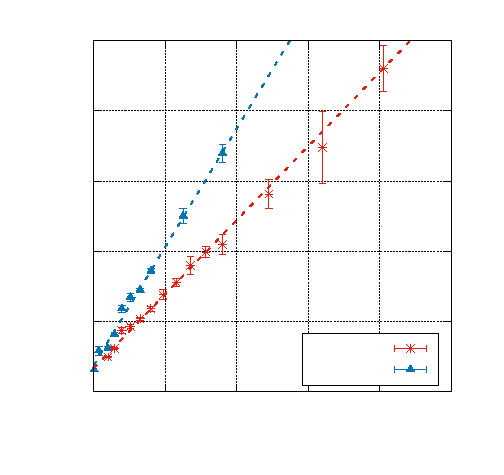
\includegraphics{water}}%
    \gplfronttext
  \end{picture}%
\endgroup

\caption{Amplitude decay rate $\mathcal{R}$ as a function of pulse
  interval squared $\tau^2$ for two different positions of a water
  sample, also linear fits to the two measurement series are
  shown. Each measurement point is given with 95\,\% confidence
  interval. The ``off mark'' sample was moved to about 1\,mm off the
  mark which was used for the rest of the (``on mark'') measurements. } 
\label{fig:water-pos}
\end{figure}

The first results of these measurements is the effect of sample
positioning inside the NMR apparatus. The result of the two
measurement series are shown in \figref{fig:water-pos}.
The parameters for the two linear fits, \eqref{eq:multi-pulse-rate},
were $R_2=\unit[0.67]{s^{-1}}$ and  
$K=\unit[4.21\times10^{-3}]{s^{-1}/ms^2}$ for the ``on mark'' water
measurements, and $R_2=\unit[0.76]{s^{-1}}$ and
$K=\unit[6.75\times10^{-3}]{s^{-1}/ms^2}$ for the ``off mark''.





\section{Discussion}
\todo[inline]{Compare $T_2$ values to that of literature.}

As mentioned in section~\ref{sec:met}, special care was taken so that
the each measurement would be as equivalent to each other as
possible. However since the devise is meant for student lab use $B_0$
(and also $\pdv*{B_0}{z}$) was strongly non-uniform, as we saw when we
tested to move the sample by just 1\,mm. This means that any
qualitative results regarding the diffusivity would be highly
unreliable. 
\todo[inline]{We therefore only consider the quantitative results.}


\todo[inline]{We also tried dry paper, but did not see anything.}


\todo[inline]{Pulses much shorter than pulse intervals, menaing that
  we don't have to worry about that. }


\section{Conclusions}

In conclusion, we only considered quantitative results due to the due to unreliability of results of diffusitivity. Experiments were done for  No results were seen in dry paper due to its molecular structure. 

%\section{References}
%http://hyperphysics.phy-astr.gsu.edu/hbase/Nuclear/nmr.html

%%%%%%%%%%%%%%%%%%%%%%%%%% The bibliography %%%%%%%%%%%%%%%%%%%%%%%%%%
\newpage
%% This bibliography uses BibTeX
\bibliographystyle{ieeetr}
\bibliography{references}%requires a file named 'references.bib'
%% Citations are as usual: \cite{example_article}

%%%%%%%%%%%%%%%%%%%%%%%%%%%%% Appendices %%%%%%%%%%%%%%%%%%%%%%%%%%%%%
\clearpage %% on a new page 
\appendix  %% This will change the page numbering to A1, A2, A3, ...;
           %% and also change the sections to A, A.1, ...; B, B.1, ...





%%%%%%%%%%%%%%%%%%%%%%%%%%%%%%%%%%%%%%%%%%%%%%%%%%%%%%%%%%%%%%%%%%%%%%
\end{document}%% ^ ^ ^ ^ ^ ^ ^ ^ ^ ^ ^ ^ ^ ^ ^ ^ ^ ^ ^ ^ ^ ^ ^ ^ ^ ^ ^
%%%%%%%%%%%%%%%%%%%%%%%%%%%%%%%%%%%%%%%%%%%%%%%%%%%%%%%%%%%%%%%%%%%%%%



%  LocalWords:  Larmor coherentness diffusivity multi Batchelor
